\documentclass[twocolumn, 8pt]{article}

\usepackage[english]{babel} 


\usepackage[utf8]{inputenc}
\usepackage[T1]{fontenc}
\usepackage{lmodern}
\usepackage{amsmath}
\usepackage{verbatim}
\usepackage{amssymb}
\usepackage{mathtools}
\usepackage{enumitem}
\usepackage{float}
\usepackage{titlesec} 

\titleformat{\subsection}[runin]{\normalfont\large\bfseries}{\thesubsection}{1em}{}

\setlength{\parindent}{0pt}

\begin{document}

\begin{center}

\Large{\textbf{MLDS: Homework 1}} \\
\textsc{\large{Andraž De Luisa}} \\
\vspace{6pt}
\small{\today}

\end{center}

Given a data set with numeric input (independent) variables $x_i$  in and binary target (dependent) $y_i$, we decide to use logistic regression: $(y_i|x_i,\beta) \sim \text{Bernoulli}(\theta_i), \text{where} ~
 \theta_i = \frac{1}{1+e^{-\beta^T x_i}}$.

\subsection*{Exercise 1} Derive the log likelihood: \\

\begin{math} 
    L(\beta, y, x) = \prod_{i=1}^n \theta_i^{y_i} (1-\theta_i)^{1-y_i} = \prod_{i=1}^n \frac{1}{1+e^{-\beta^T x_i}}^{y_i} \cdot \\
    \cdot \Big(1-\frac{1}{1+e^{-\beta^T x_i}}\Big)^{1-y_i} = \prod_{i=1}^n \frac{e^{-\beta^T x_i (1-y_i)}}{1+e^{-\beta^T x_i}}
\end{math}

\begin{math}
    l(\beta, y, x) = \sum_{i=1}^n -\beta^T x_i (1-y_i) - \log{(1 + e^{-\beta^T x_i})}
\end{math}

\subsection*{Exercise 3b} Derive the gradient of the log-likelihood: \\

\begin{math}
    \frac{\delta}{\delta \beta} l(\beta, y, x) = \sum_{i=1}^{n} -x_i^T (1-y_i) + \frac{x_i e^{-\beta^T x_i}}{1 + e^{-\beta^T x_i}} = \sum_{i=1}^{n} x_i \Big(y_i - 1 + \frac{e^{-\beta^T x_i}}{1 + e^{-\beta^T x_i}} \Big) = \\ 
    = \sum_{i=1}^{n} x_i \Big(y_i - \frac{1}{1 + e^{-\beta^T x_i}}\Big)
\end{math} \\

The number of function calls before the optimization was varying between 5000 and 25000 (depending on the degree of polynomial expansion), while after the optimization it stabilized around 20.

\subsection*{Exercise 5} Before the application of logistic regression I normalized the data in the 'housing' dataset, because the intervals in which data in different columns were lying were too much different between them. The 'painted' dataset was already normalized on the [0,1] interval. \\

In figures \ref{fig:paint} and \ref{fig:house} the misclassification rates with respect to the growth of the degree of polynomial expansion of the dataset features are shown. Both plots show a similar pattern of overfitting the training data after some time, which is expected since the number of data instances in the datasets is substantially smaller than the number of features in an expanded dataset of degree 4 or more. Still, the logistic regression in the 'housing' dataset is quite stable if we compare it to the 'painted' dataset, its double size does probably help here.

\begin{figure}[ht]
    \centering
    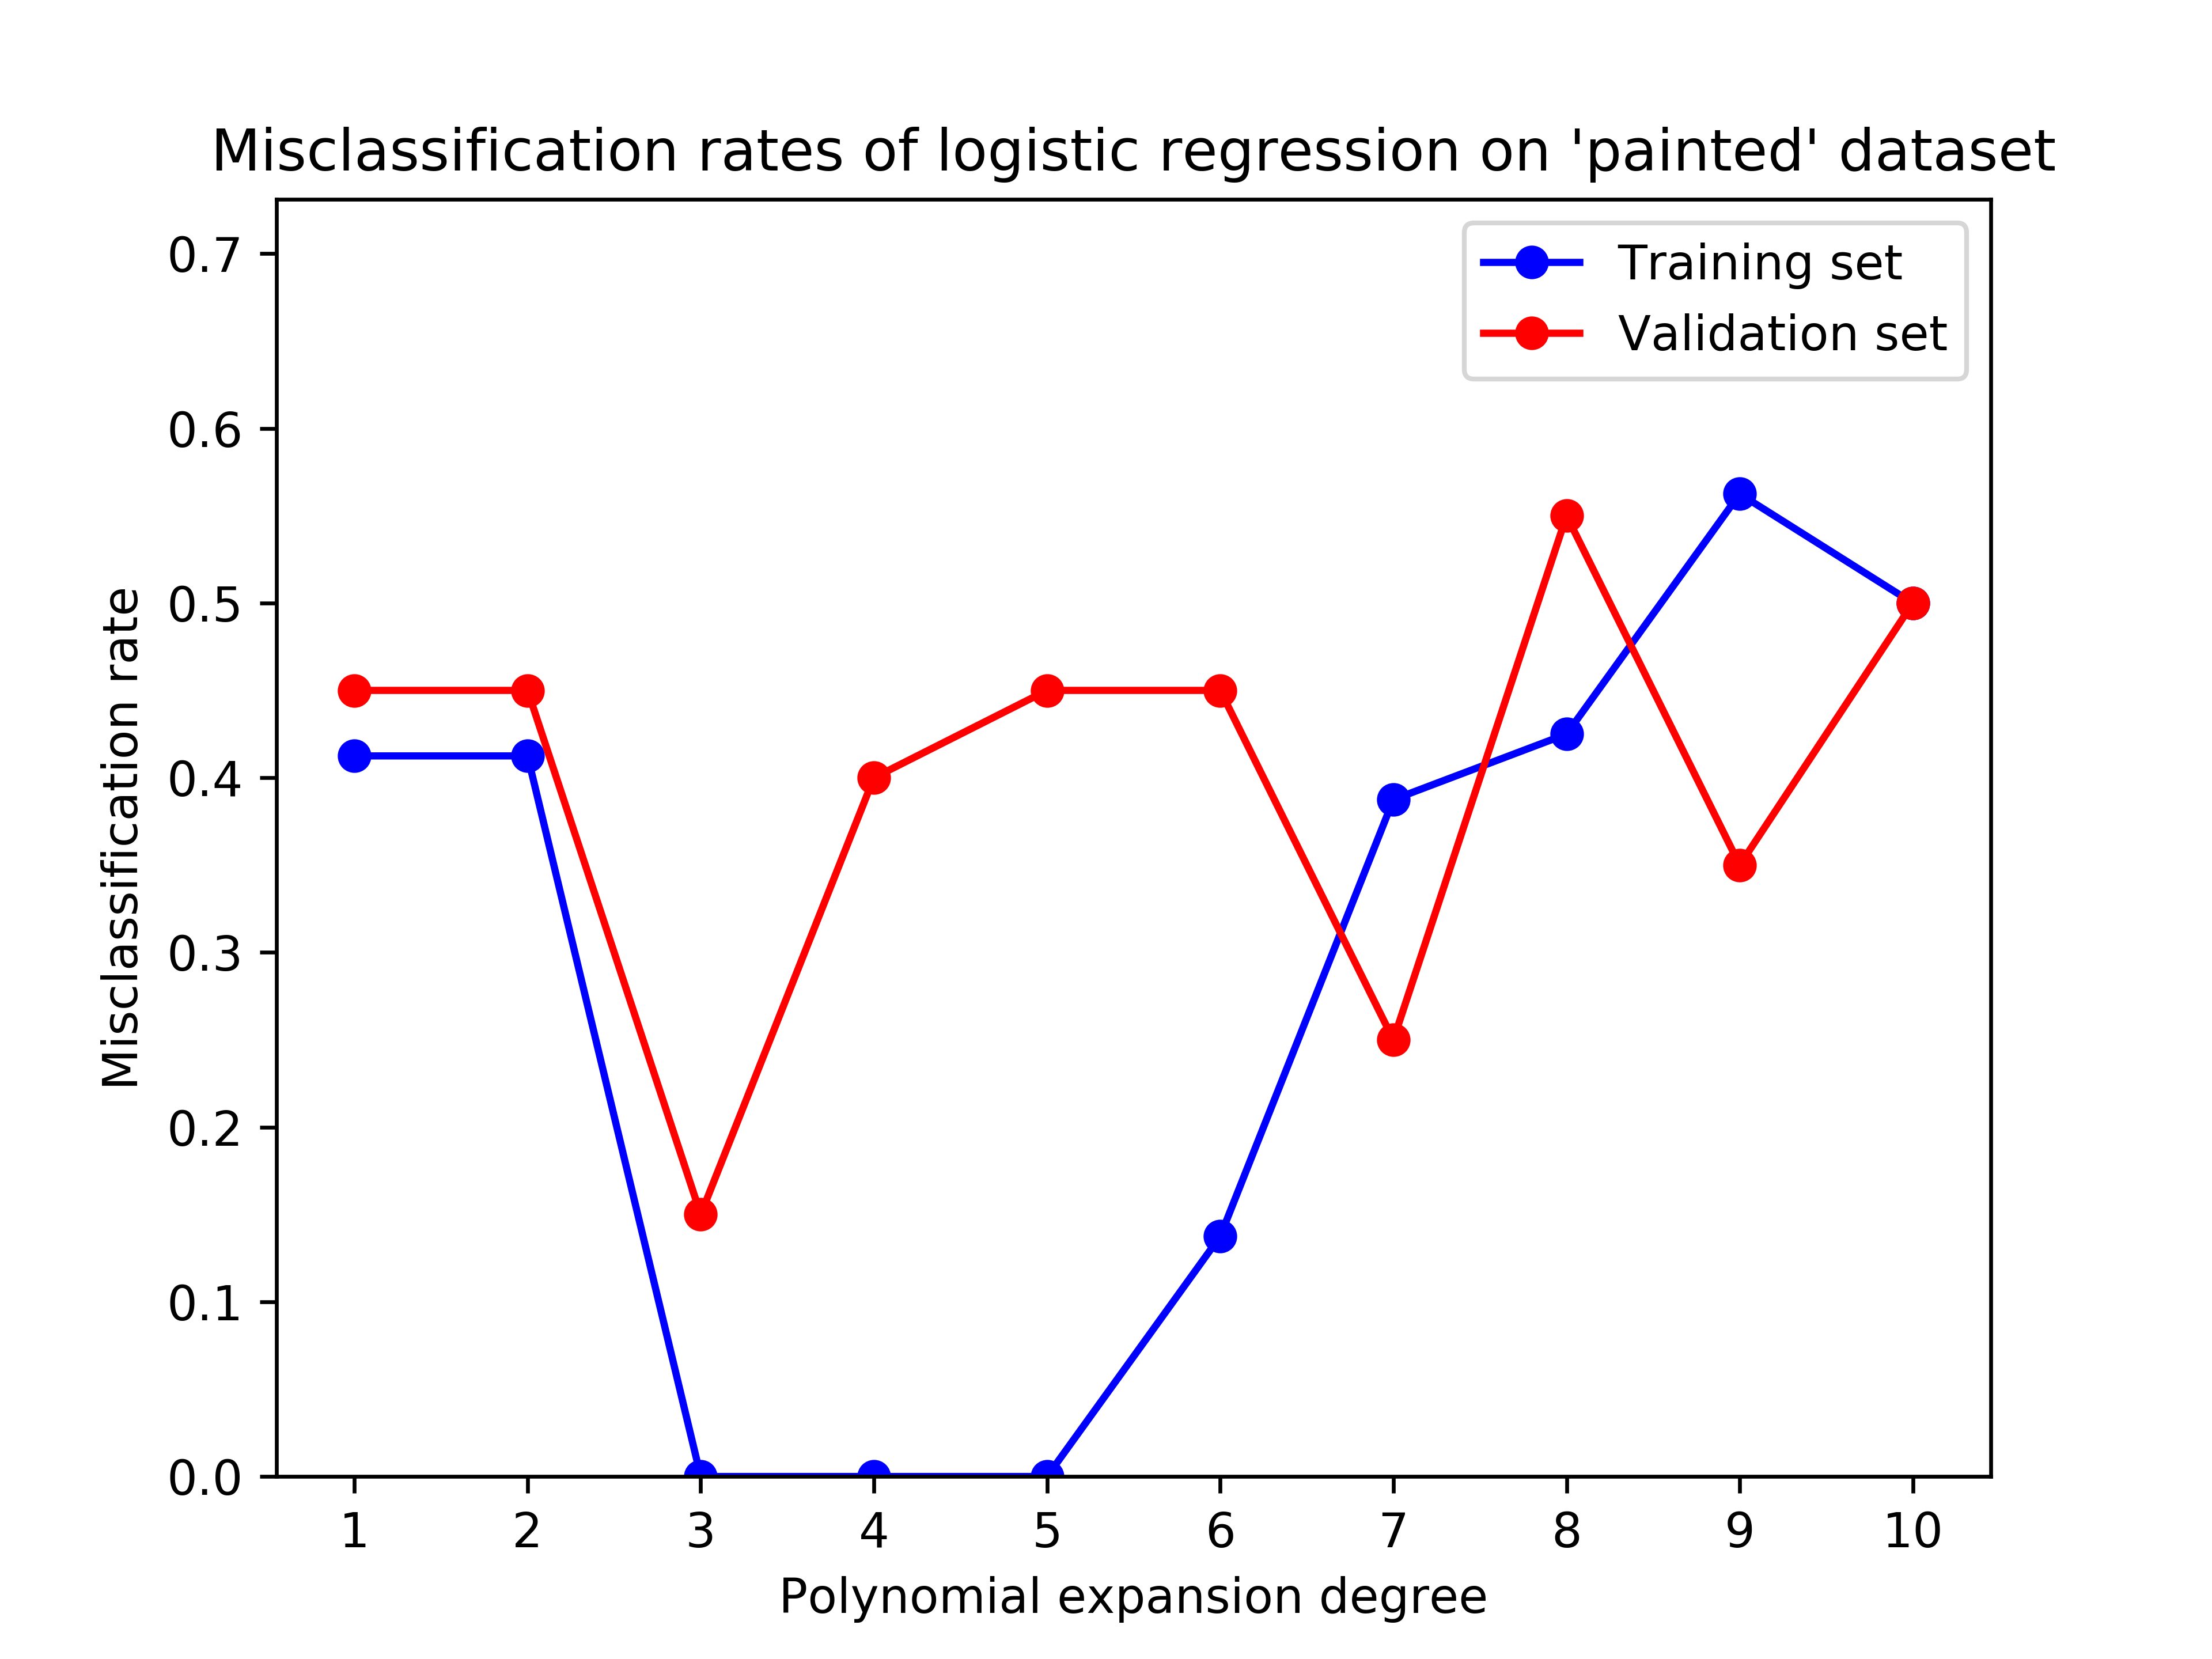
\includegraphics[width=.45\textwidth]{painted2.png}
    \caption{Changes of misclassification rates with respect to the polynomial expansion degree of the 'painted' dataset.}
    \label{fig:paint}
    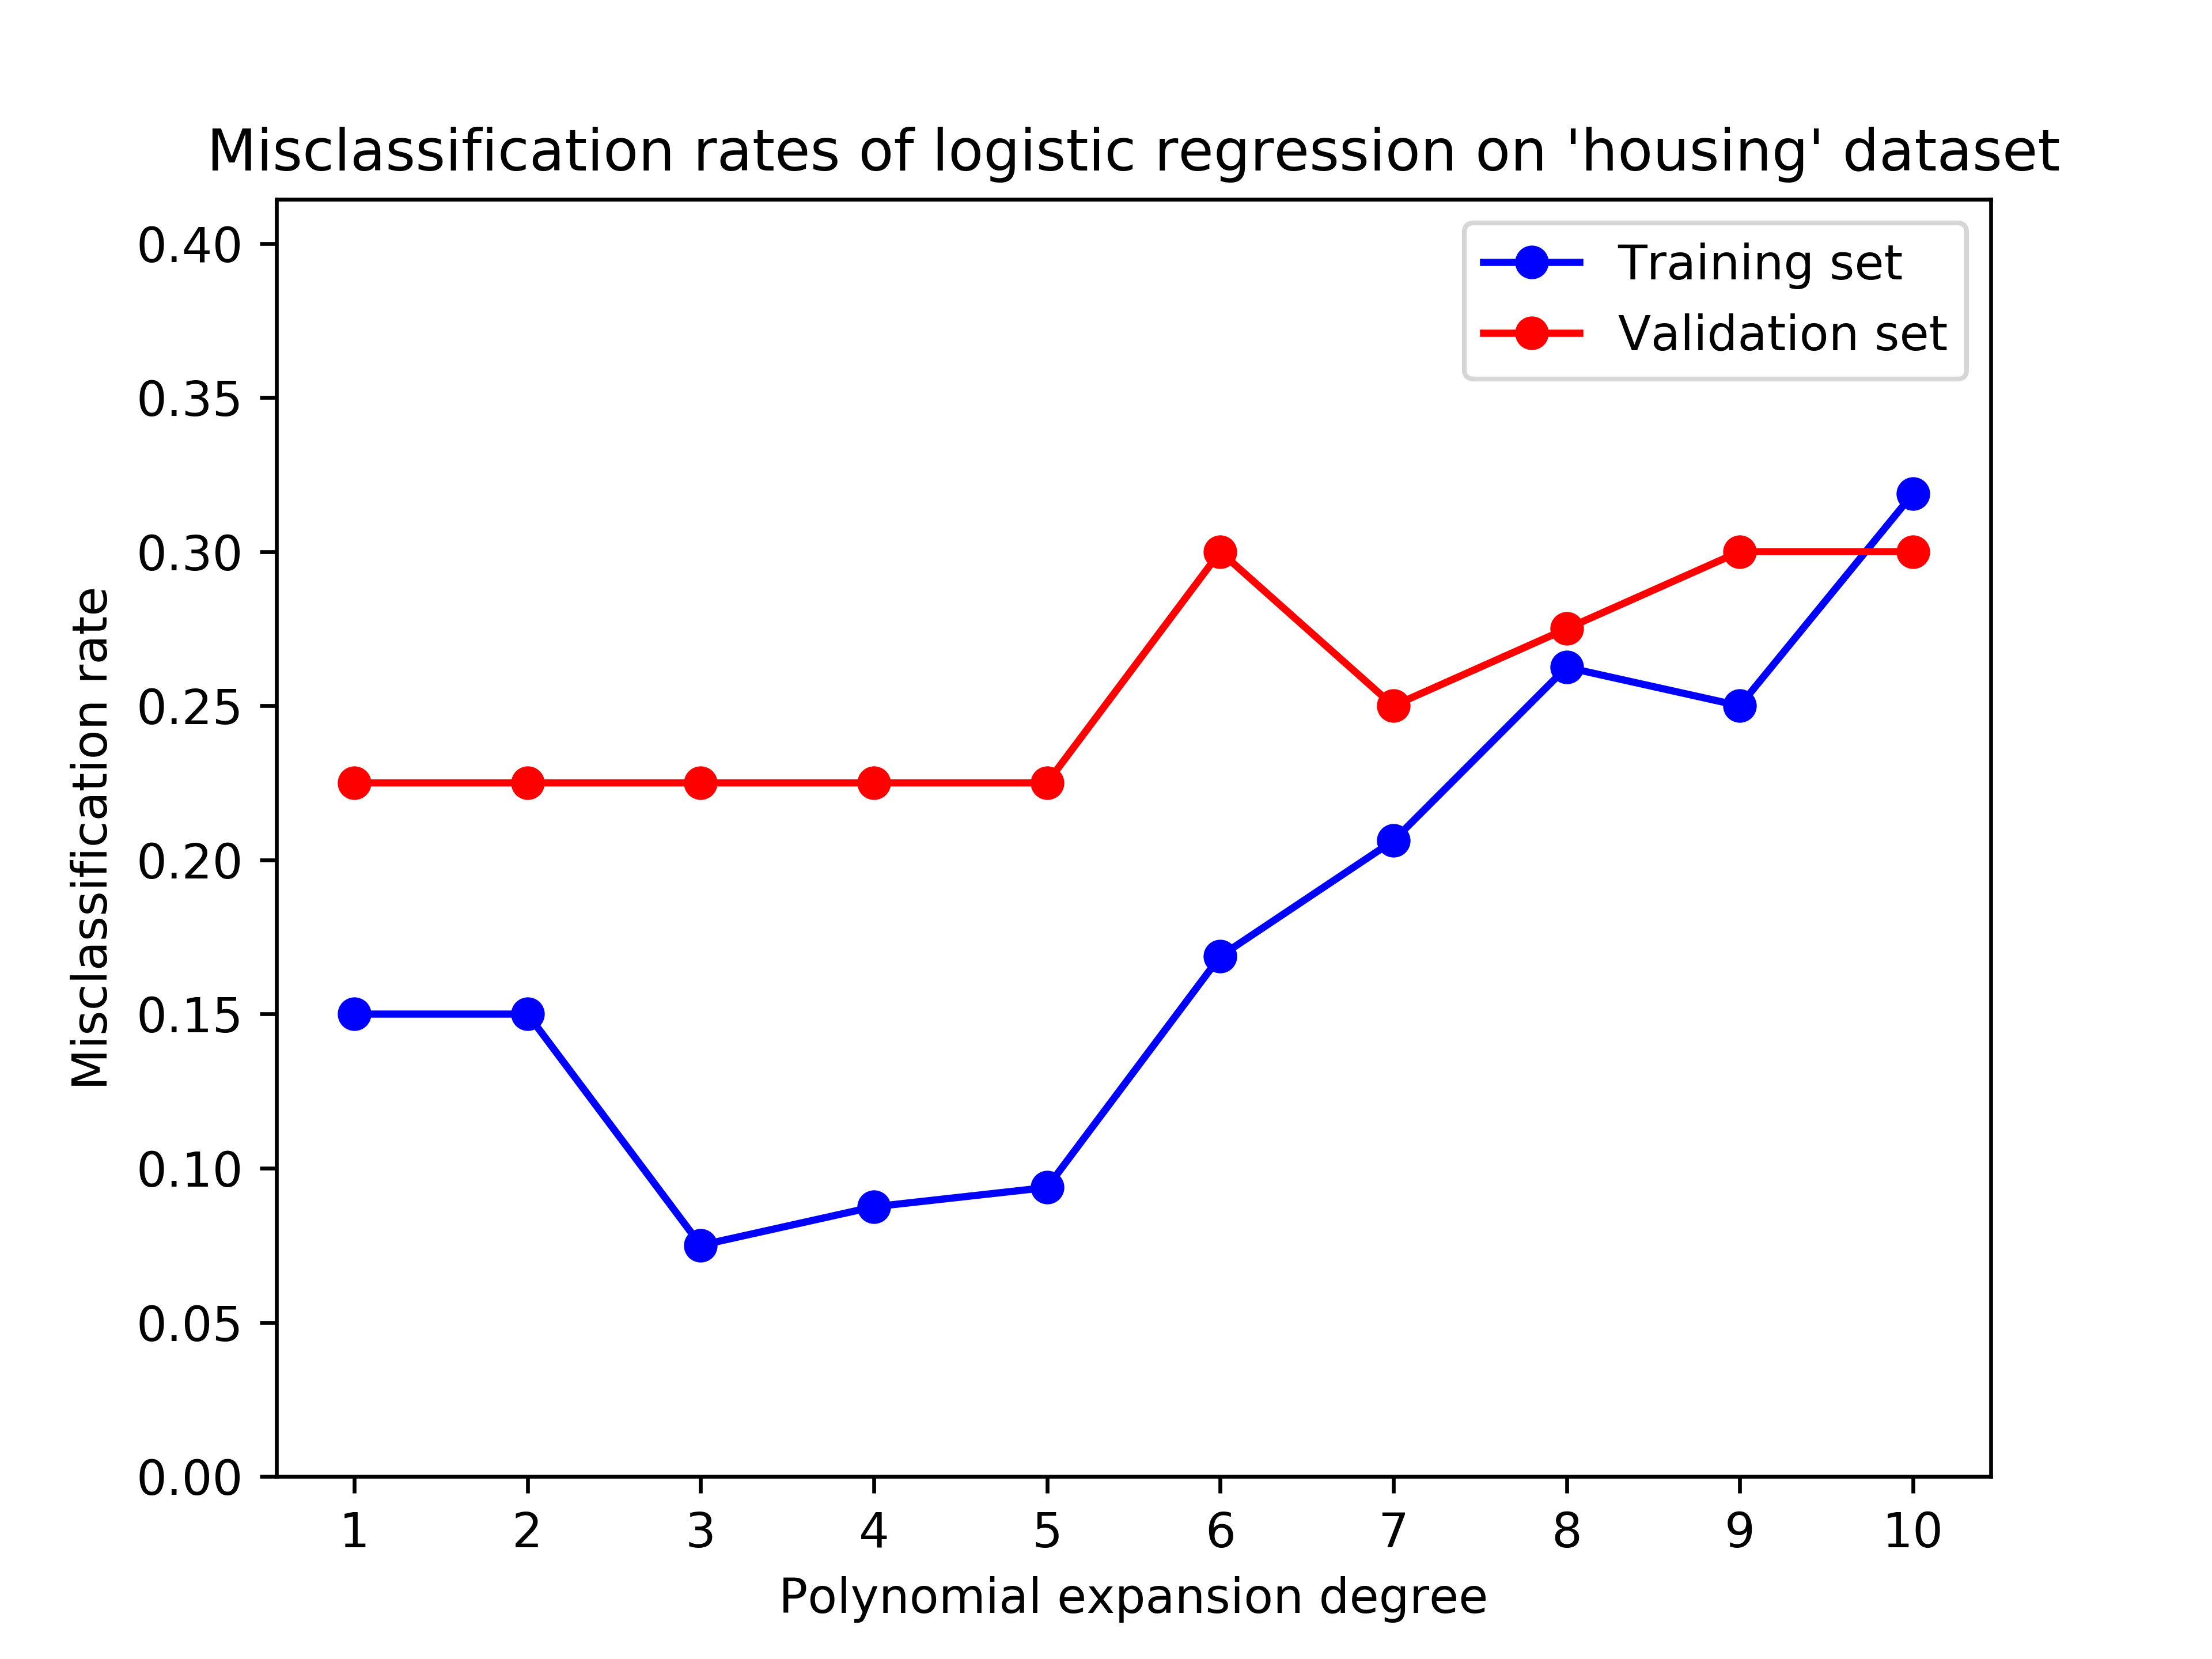
\includegraphics[width=.45\textwidth]{housing2.png}
    \caption{Changes of misclassification rates with respect to the polynomial expansion degree of the 'housing' dataset.}
    \label{fig:house}
\end{figure}

\end{document}